\section{Senkrechte Geraden und Anwendungen}
Im diesem Abschnitt geht es um verschiedene Anwendungen, wo zwei lineare Funktionen im Spiel sind.
\subsection{Parallele Geraden}
\begin{fazit}[]{}
    Zwei Geraden sind parallel, wenn ihre Steigungen gleich sind.
\end{fazit}
\begin{example}
    Bestimmen Sie die Gleichung derjenigen Funktion, welche parallel zu $f:y=-5x+2$ ist und durch den Punkt $P=(-2,3)$ geht.\\
    \bigskip

    \textbf{Lösung:} Da die gesuchte Funktion parallel zu $f$ sein soll, hat sie dieselbe Steigung:
    \begin{align*}
        g(x) = -5x + b
    \end{align*}
    Um den $y$-Achsenabschnitt $b$ zu bestimmen, setzen wir den Punkt $P$ in die Gleichung von $g$ ein:
    \begin{align*}
        3 & = -5\cdot 2 + b \\
        b & = 13
    \end{align*}
    Also lautet die Gleichung der gesuchten Funktion:
    \begin{align*}
        g(x) = -5x + 13
    \end{align*}
\end{example}
\newpage

\subsection{Schnittpunkte zweier Geraden}
\begin{minipage}{0.4\textwidth}
    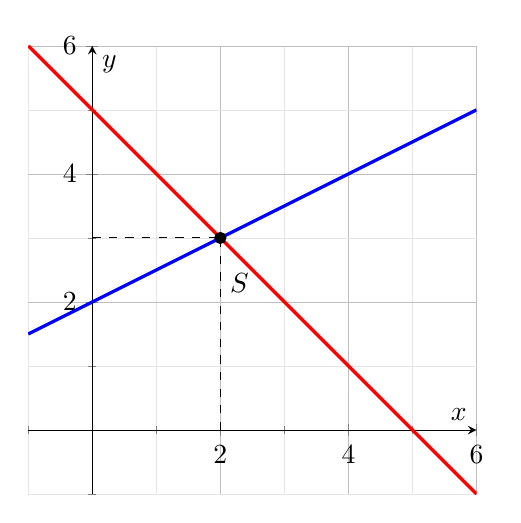
\begin{tikzpicture}
        \begin{axis}[
                axis lines = middle,
                xlabel = $x$,
                ylabel = $y$,
                xmin=-1, xmax=6,
                ymin=-1, ymax=6,
                grid=both,
                minor tick num=1,
                major grid style={line width=.2pt,draw=gray!50},
                minor grid style={line width=.1pt,draw=gray!20},
                domain=-1:6,
                samples=100,
                axis equal image,
                legend style={at={(0.02,0.98)}, anchor=north west}
            ]

            % f(x) = 0.5x + 1
            \addplot[very thick, blue] {0.5*x + 2};

            % g(x) = -x + 4
            \addplot[very thick, red] {-1*x + 5};

            % Schnittpunkt S(2,2)
            \addplot[
                only marks,
                mark=*,
                mark size=2pt
            ] coordinates {(2,3)};

            % Beschriftung des Schnittpunkts
            \node at (axis cs:2,2) [anchor=south west] {$S$};

            % Hilfslinien vom Schnittpunkt zu den Achsen
            \draw[dashed] (axis cs:2,0) -- (axis cs:2,3);
            \draw[dashed] (axis cs:0,3) -- (axis cs:2,3);

        \end{axis}
    \end{tikzpicture}
\end{minipage}\begin{minipage}
    {0.55\textwidth}
    Der Schnittpunkt $S$ zweier Geraden ist der Punkt, der auf beiden Funktionsgraphen liegt. In diesem Punkt haben beide Funktionen denselben $x$- und $y$-Wert. Um den Schnittpunkt zu berechnen, setzt man also die beiden Funktionsterme gleich und löst nach $x$ auf. Der so gefundene $x$-Wert wird in eine der beiden Gleichungen eingesetzt, um den zugehörigen $y$-Wert zu erhalten.
\end{minipage}

\begin{fazit}[]{}
    Den Schnittpunkt zweier Geraden erhält man, indem man ihr Funktionsterme gleichsetzt und nach der Variablen $x$ auflöst.
\end{fazit}
\begin{example}
    Bestimmen Sie den Schnittpunkt von $f:y = -3x + 2$ und $g: y = 2x -3$.\\
    \bigskip

    \textbf{Lösung:}
    \begin{align*}
        -3x + 2 & = 2x - 3                  \\
        5x      & = 5                       \\
        x       & =1                        \\
        y       & = g(1) = 2\cdot 1 -3 = -1
    \end{align*}
    Also $S=(1,-1)$
\end{example}
\newpage
\subsection{Senkrechte Geraden}
\begin{example}
    \begin{align*}
        f :y=-\dfrac{2}{3} x+1,\ g:y=\dfrac{3}{2} x-1
    \end{align*}
    Wenn man $f$ und $g$ in ein Koordinatensystem einzeichnet, liegt die Vermutung nahe, dass die beiden Geraden senkrecht aufeinander stehen:
    \begin{center}
        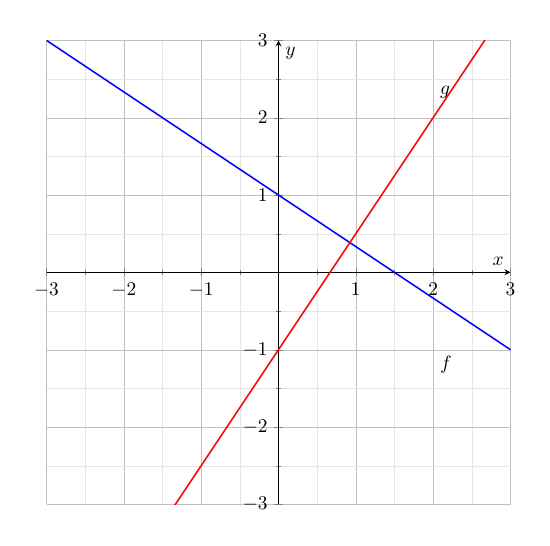
\begin{tikzpicture}[scale=0.7]
            \begin{axis}[
                    axis lines = middle,
                    xlabel = $x$,
                    ylabel = $y$,
                    ymin=-3, ymax=3,
                    xmin=-3, xmax=3,
                    grid=both,
                    minor tick num=1,
                    major grid style={line width=.2pt,draw=gray!50},
                    minor grid style={line width=.1pt,draw=gray!20},
                    width=10cm,
                    height=10cm,
                    domain=-3:3,
                    samples=100
                ]
                \addplot[blue, thick] {-2/3*x + 1};
                \addplot[red, thick] {3/2*x - 1};
                \node at (axis cs:2,-1) [anchor=north west] {$f$};
                \node at (axis cs:2,2.5) [anchor=north west] {$g$};
            \end{axis}
        \end{tikzpicture}
    \end{center}
    Betrachten wir zunächst $f$ und den um $90^\circ$ nach rechts gedrehten Graphen von $f$. Wir zeichnen ein Steigungsdreieck ein und drehen dies ebenfalls um $90^\circ$ nach links:
    \begin{center}
        \begin{minipage}{0.5\textwidth}
            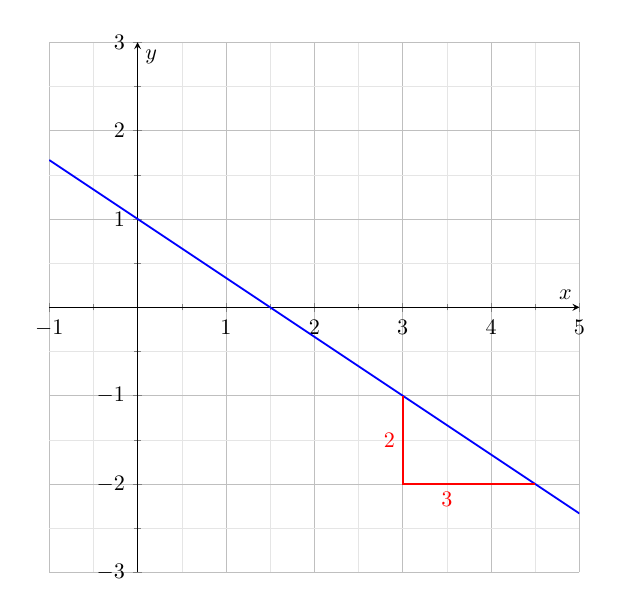
\begin{tikzpicture}[scale=0.8]
                \begin{axis}[
                        axis lines = middle,
                        xlabel = $x$,
                        ylabel = $y$,
                        ymin=-3, ymax=3,
                        xmin=-1, xmax=5,
                        grid=both,
                        minor tick num=1,
                        major grid style={line width=.2pt,draw=gray!50},
                        minor grid style={line width=.1pt,draw=gray!20},
                        width=10cm,
                        height=10cm,
                        domain=-1:5,
                        samples=50
                    ]
                    \addplot[blue, thick] {-2/3*x + 1};
                    \draw[red, thick] (3,-1) -- (3,-2) -- (4.5,-2);
                    \node at (axis cs:3,-1.5) [anchor=east, color=red] {$2$};
                    \node at (axis cs:3.5,-2) [anchor=north, color=red] {$3$};
                \end{axis}
            \end{tikzpicture}
        \end{minipage}\begin{minipage}{0.5\textwidth}
            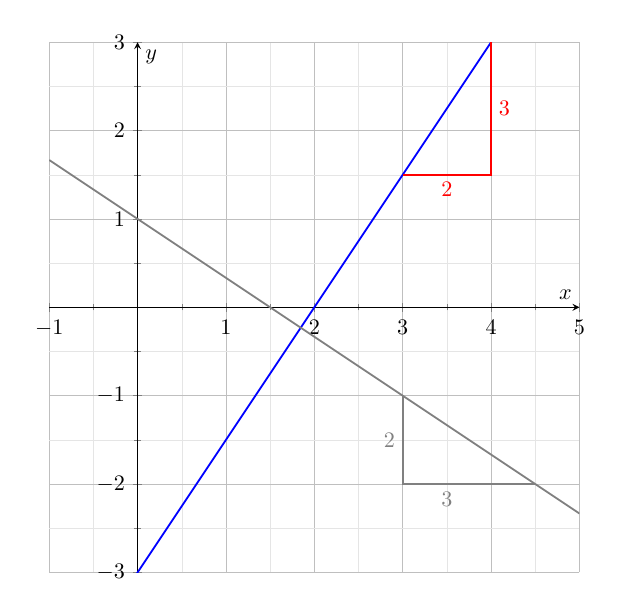
\begin{tikzpicture}[scale=0.8]
                \begin{axis}[
                        axis lines = middle,
                        xlabel = $x$,
                        ylabel = $y$,
                        ymin=-3, ymax=3,
                        xmin=-1, xmax=5,
                        grid=both,
                        minor tick num=1,
                        major grid style={line width=.2pt,draw=gray!50},
                        minor grid style={line width=.1pt,draw=gray!20},
                        width=10cm,
                        height=10cm,
                        domain=-1:5,
                        samples=50
                    ]
                    \addplot[blue, thick] {3/2*x -3};
                    \draw[red, thick] (4,3) -- (4,1.5) -- (3,1.5);
                    \node at (axis cs:4,2.25) [anchor=west, color=red] {$3$};
                    \node at (axis cs:3.5,1.5) [anchor=north, color=red] {$2$};

                    \addplot[gray, thick] {-2/3*x + 1};
                    \draw[gray, thick] (3,-1) -- (3,-2) -- (4.5,-2);
                    \node at (axis cs:3,-1.5) [anchor=east, color=gray] {$2$};
                    \node at (axis cs:3.5,-2) [anchor=north, color=gray] {$3$};
                \end{axis}
            \end{tikzpicture}
        \end{minipage}
    \end{center}
    Man erkennt, dass $\Delta y = 2$ und $\Delta x=3$ vertauscht wurden. Im gedrehten Graphen ist nun $\Delta y =3$ und $\Delta x = 2$.

    Die Steigung ist von einer negativen Steigung zu einer positiven Steigung gewechselt. Insgesamt ergibt sich also:
    \begin{align*}
        m_f                   & = -\dfrac{2}{3} \\
        m_{f\ \text{gedreht}} & = \dfrac{3}{2}
    \end{align*}
\end{example}
\begin{fazit}[]{}
    Zwei Geraden $f:y=m_f\cdot x+q$ und $g:y=m_g\cdot x+q$ sind senkrecht zueinander, wenn die eine Steigung der anderen Steigung mit dem negativen Kehrwert entspricht:
    \begin{align*}
        m_f =-\dfrac{1}{m_g}
    \end{align*}
\end{fazit}
\begin{example}
    Die Geraden $f:y=-4x+1$ und $g:y=\dfrac{1}{4}x-2$ stehen senkrecht zueinander, weil:
    \begin{align*}
        m_f             & = -4                                  \\
        -\dfrac{1}{m_g} & = -\dfrac{1}{\dfrac{1}{4}} = -4 = m_f
    \end{align*}
\end{example}
\begin{example}
    Bestimmen Sie die Gleichung derjenigen Funktion $g$, welche senkrecht zu $f:y= \dfrac{2}{5} x +3$ ist und durch den Punkt $P=(6,4)$ geht.
    \kariert{28}
\end{example}
\newpage
\subsection*{Abstand zweier Punkte}
\begin{example}
    Wir berechnen den Abstand $|AB|$ der Punkte $A=(-2,4)$ und $B=(3,7)$.

    \begin{minipage}{0.45\textwidth}
        \begin{center}
            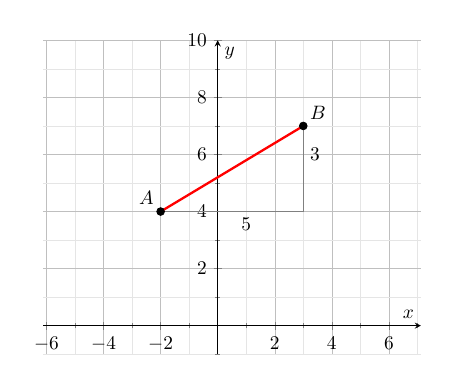
\begin{tikzpicture}[scale=0.7]
                \begin{axis}[
                        axis lines = middle,
                        xlabel = $x$,
                        ylabel = $y$,
                        ymin=-1, ymax=10,
                        xmin=-4, xmax=5,
                        grid=both,
                        minor tick num=1,
                        major grid style={line width=.2pt,draw=gray!50},
                        minor grid style={line width=.1pt,draw=gray!20},
                        axis equal,
                    ]
                    \addplot[only marks, mark=*, mark size=2pt] coordinates {(-2,4) (3,7)};
                    \node at (axis cs:-2,4) [anchor=south east] {$A$};
                    \node at (axis cs:3,7) [anchor=south west] {$B$};
                    \draw[red, very thick] (-2,4) -- (3,7);
                    \draw[gray] (-2,4) -- (3,4) -- (3,7);
                    \node at (axis cs:1,4) [anchor=north, color=black] {$5$};
                    \node at (axis cs:3,6) [anchor=west, color=black] {$3$};
                \end{axis}
            \end{tikzpicture}
        \end{center}
    \end{minipage}\begin{minipage}
        {0.45\textwidth} Wir zeichnen die Punkte $A$ und $B$ in ein Koordinatensystem ein. Zusätzlich zeichnen wir noch das Steigungsdreieck der Gerade durch $A$ und $B$ ein. Dies ist ein rechtwinkliges Dreieck mit den Katheten $3$ und $10$.
    \end{minipage}
    \smallskip

    Mit dem Satz des Pythagoras erhalten wir:
    \begin{align*}
        |AB| & = \sqrt{3^2 + 5^2} = \sqrt{34} \approx 5.83
    \end{align*}
\end{example}

\begin{example}
    Berechnen Sie den Abstand der Punkte $A=(1,2)$ und $B=(7,5)$.

    Wir berechnen zuerst die Seiten des Steigungsdreiecks:
    \begin{align*}
        \Delta x & = 7 - 1 = 6 \\
        \Delta y & = 5 - 2 = 3
    \end{align*}
    Mit dem Satz des Pythagoras erhalten wir:
    \begin{align*}
        |AB| & = \sqrt{6^2 + 3^2} = \sqrt{45} \approx 6.71
    \end{align*}
\end{example}
\newpage
\subsection{Anwendungsaufgaben}
\subsubsection*{Punkte auf Gerade?}
Liegen die Punkte $A(1,-2)$, $B(5,2)$ und $C(10,5)$ auf einer Geraden?
\kariert{40}
\newpage
\subsubsection*{Rechteck gesucht}
Gesucht sind die Koordinaten der Ecken des Rechtecks $ABCD$, wobei
\begin{itemize}
    \item $C=(3,7)$
    \item $|AB|= 5$ und
    \item $AB$ liegt auf der Geraden $g: y = \dfrac{3}{4}x -7.75$
\end{itemize}
\kariert{40}
\newpage
\subsubsection*{Quadrat?}
Bilden die Schnittpunkte der folgenden Funktionen ein Quadrat?
\begin{align*}
    f:y=2x+3                        &  &
    g:y=2x-3                             \\
    h:y=-\dfrac{1}{2}x-\dfrac{3}{2} &  &
    k:y=-\dfrac{1}{2}x+\dfrac{3}{2}
\end{align*}
\kariert{40}
\newpage
\subsubsection*{Abstand Punkt - Gerade}
Gegeben ist der Punkt $A=(3,5)$ und die Gerade $g:y=0.4x-2$. Welchen Abstand hat der Punkt $A$ von der Geraden $g$?
\kariert{40}
\newpage
\subsection{Aufgaben}
\begin{enumerate}
    \item Gegeben ist der Punkt $A=(3,-9)$ und die Gerade $g:y=-0.2x+2$.
          \begin{enumerate}
              \item Welchen Abstand hat der Punkt $A$ von der Geraden $g$?
              \item Welche Koordinaten hat der Bildpunkt $A'$, wenn $A$ an $g$ gespiegelt wird?
          \end{enumerate}
    \item Berechnen Sie den Abstand der Geraden $g:4x+3y=30$ vom Ursprung.
    \item Berechnen Sie den Abstand der beiden parallelen Geraden $g:y=\dfrac{4}{3}x-5$ und $h:y=\dfrac{4}{3}x+10$.
    \item Berechnen Sie die Länge der Höhe $h_a$ des Dreiecks $\triangle ABC$, wobei $A=(-3,4)$, $B=(-4,3-)$ und $C=(8,6)$.
    \item Richtig oder falsch.
          \begin{enumerate}
              \item Das Produkt der Steigungen zweier senkrechter Geraden ist $-1$.
              \item Der Abstand zweier parallelen Geraden ist der Unterschied der beiden y-Achsenabschnitte.
              \item Die Steigung einer vertikalen Gerade ist stets $100\%$.
              \item Die Steigung eines steilen Bergweges beträgt $45\%$. Dargestellt in einem Koordinatensystem entspricht dies einer Steigung von $\dfrac{9}{20}$.
          \end{enumerate}
\end{enumerate}
\vspace{10cm}

\subsubsection{Lösungen}
\begin{multicols}{2}
    \begin{enumerate}
        \item \begin{enumerate}
                  \item $\sqrt{104}$
                  \item $A'=(7,11)$
              \end{enumerate}
        \item $6$
        \item $9$
        \item $5$
        \item \begin{enumerate}
                  \item Richtig
                  \item Falsch
                  \item Falsch
                  \item Richtig
              \end{enumerate}
    \end{enumerate}
\end{multicols}